\section{Exercises}\label{4_4_exercises}
%should have predefined exercises that can be tracked in an appropriate manner
Each exercise is part of one stage. An exercise itself is divided into two body sides, which are further divided into several repetitions, see figure \ref{fig:exerciseStructure}. Every exercise is locked except the first one to provide a starting point, like with the stages. The next exercise should be unlocked by accomplishing both sides of the current exercise. Similarly a side will be completed if all repetitions have been finished. Like for the stage, each exercise should be instructed for the user, such that she can successfully perform it. The system will also recognise if the user is ready to start with the exercise. During the execution she should get real time feedback about her current performance. An exercise summary should show the performance of the execution with several performance parameters regarding the given gesture.

\begin{figure}[htb]
	\centering
	\begin{minipage}[t]{1\linewidth}
		\centering
		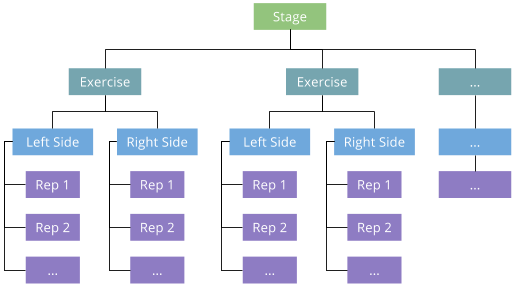
\includegraphics[width=1\linewidth]{Pictures/exerciseStructureTopDown2}
		\caption{Exercise structure}
		\label{fig:exerciseStructure}
	\end{minipage}
\end{figure}
\begin{comment}
\\- system should provide predefined exercises that can be tracked per user
\\- A stage menu should be provided to the user, which shows her the amount of stages to complete
\\- It consists of 4 stages each with specific exercises (Preliminary, First contact with slacklining,  Static exercises, Dynamic exercises) like explained in chapter 3
\\- A stage consists of several exercises like explained in prev. chapter
\\- locked stages (initial first stage interactable)
\\- unlock stages (by successfully accomplishing all exercises from current stage)
\\- Stage introduction gives general information, describes the goal and tips for the current stage
-- a stage information scene provides her with the general introduction of this stage --> unlocks first exercise
\\- Stage summary contains average data about each exercise
\end{comment}
